\chapter{Introducción específica} % Main chapter title

\label{Chapter2}

%----------------------------------------------------------------------------------------
%	SECTION 1
%----------------------------------------------------------------------------------------
En este capítulo se describen las tecnologías, herramientas y protocolos utilizados para la realización del trabajo.

\section{Tecnologías de comunicación}
\label{sec:Tecnologías de comunicación}
A continuación se describen los principales protocolos empleados en el trabajo. En la figura \ref{fig:IotProtocols} se observa su posicionamiento en la pila de protocolos para IoT.

\begin{figure}[h]
	\centering
	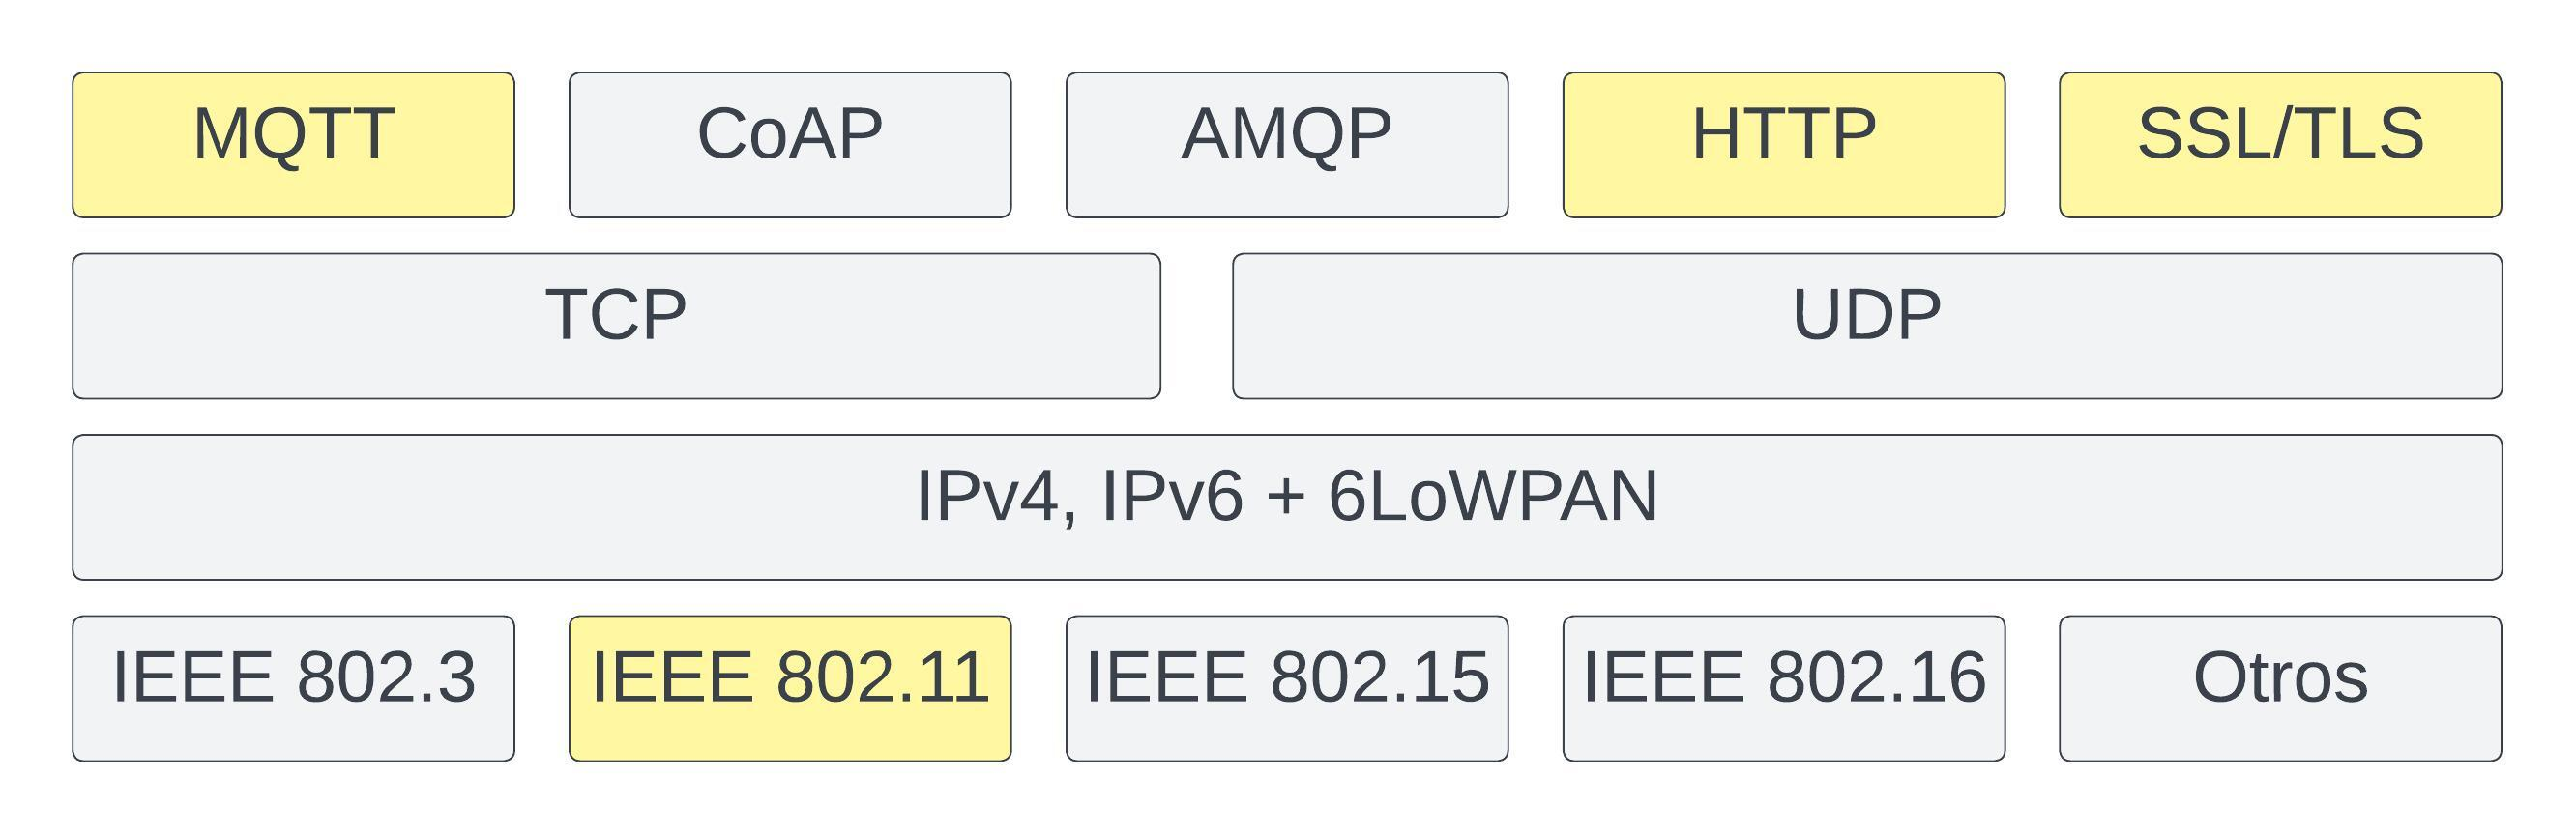
\includegraphics[width=0.75\textwidth]{./Figures/protocols.jpeg}
	\caption[Pila de protocolos para IoT.]{Pila de protocolos para IoT\protect\footnotemark.}
	\label{fig:IotProtocols}

\end{figure}
	\footnotetext{Gráfico creado en base a una imagen tomada de: \citep{8088251}.}

\subsection{Tecnologías Wi-Fi}
\label{sec:Tecnologías Wi-Fi}
El estándar IEEE 802.11 para redes inalámbricas de área local (WLAN) es conocido comercialmente como Wi-Fi. Este estándar presenta dos modos de operación \citep{wifi}
\begin{itemize}
\item Infraestructura: uno o máa \textit{access points} (AP) actúan como puente entre la red cableada y la red inalámbrica. Todas las comunicaciones entre los dispositivos conectados a la red, se realizan a través de los APs. 
\item Ad-hoc: cada nodo puede realizar una conexión directa con otro, sin necesidad de un AP central. Para lograr esto, los nodos se organizan en una red donde todos son capaces de enrutar los paquetes.  
\end{itemize}

\subsection{Protocolo MQTT}
\label{sec:Protocolo MQTT}

El protocolo MQTT fue desarrollado en 1999 con el objetivo principal de crear un protocolo muy eficiente desde el punto de vista del uso del ancho de banda y de muy bajo consumo de energía. Por estas razones es adecuado para el uso en IoT \citep{mqtt:1}.\\
El protocolo MQTT se basa en el paradigma de publicación-suscripción. Este paradigma desvincula un cliente que publica un mensaje o publicador de otros clientes que reciben el mensaje o suscriptores. Sumado a esto, 
MQTT es un protocolo de mensajería asincrónico, lo que significa que no frena al cliente mientras espera por el mensaje. \\ 
Un componente principal del protocolo es el \textit{broker}, su función principal es la de recibir los mensajes de los publicadores y enviarlos  a los clientes suscriptores. Para realizar esta tarea, el \textit{broker} utiliza temas o \textit{topics} para filtrar a los clientes que recibirán el mensaje. De esta manera, el \textit{topic} es un canal virtual que conecta a los publicadores con sus suscriptores \citep{mqtt:1}.

\begin{figure}[h]
	\centering
	\includegraphics[width=0.75\textwidth]{./Figures/mqtt.jpeg}
	\caption[Arquitectura del protocolo MQTT.]{Arquitectura del protocolo MQTT\protect\footnotemark.}
	\label{fig:IotProtocols}

\end{figure}

	\footnotetext{Gráfico creado en base a una imagen tomada de: \citep{mqtt:1}.}


\subsection{Protocolo HTTP}
\label{sec:Protocolo HTTP}

El \textit{Hypertext Transfer Protocol} (HTTP)\citep{http:1} es un protocolo utilizado en la web para el desarrollo de aplicaciones basado en el paradigma cliente-servidor mediante un modelo de \textit{request/response}. En los últimos tiempos se ha asociado a HTTP con la arquitectura REST (\textit{Representational State Transfer})\citep{rest} para facilitar la interacción entre distintas entidades sobre servicios basados en red. Esta asociación permite que los dispositivos interactúen mediante funciones estandares de CRUD (\textit{create, read, update, delete}\citep{10.1145/3292674}. Las funciones de CRUD son mapeadas a los métodos Post, Get, Put y Delete de HTTP respectivamente \citep{GLAROUDIS2020107037}. 

\subsection{Protocolo SSL/TLS}
\label{sec:Protocolo SSL/TLS}
\textit{Secure Socket Layer/Transport Layer Security} (SSL/TLS) \citep{tls:1} es un protocolo criptográfico que proporciona seguridad de extremo a extremo de los datos enviados entre aplicaciones a través de Internet.
TLS evolucionó a partir de \textit{Secure Socket Layers} (SSL), que fue desarrollado originalmente por Netscape Communications Corporation en 1994 para proteger las sesiones web. SSL 1.0 nunca se lanzó públicamente, mientras que SSL 2.0 fue reemplazado rápidamente por SSL 3.0 en el que se basa TLS.\\

Cabe señalar que TLS no protege los datos en los sistemas finales, simplemente asegura la entrega segura de datos a través de Internet, evitando posibles escuchas y/o alteración del contenido.
TLS normalmente se implementa sobre TCP \citep{rfc793} para cifrar los protocolos de la capa de aplicación, como por ejemplo sobre HTTP.

TLS utiliza una combinación de criptografía simétrica y asimétrica, ya que proporciona un buen compromiso entre rendimiento y seguridad cuando se transmiten datos de forma segura \citep{tls:2}. Para mayor seguridad es deseable que un cliente que se conecta a un servidor pueda validar la veracidad de la clave pública del servidor. Esto normalmente se lleva a cabo utilizando un certificado digital X.509 \citep{x509:1} emitido por un tercero de confianza conocido como Autoridad Certificadora (CA) que afirma la autenticidad de la clave pública. En algunos casos, un servidor puede usar un certificado autofirmado en el que el cliente debe confiar explícitamente \citep{tls:2}.

En la figura \ref{fig:ssl2way} se detalla el esquema de autenticación mutua entre dos dispositivos mediante la verificación del certificado presentado.

\begin{figure}[h]
	\centering
	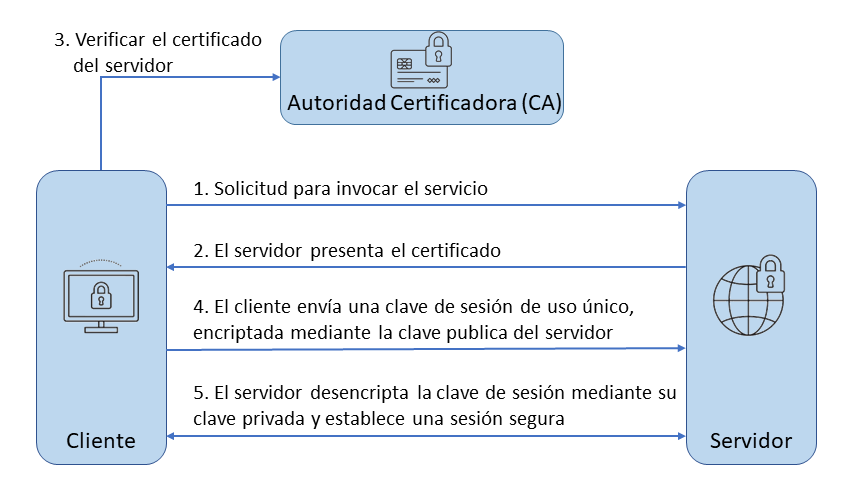
\includegraphics[width=0.75\textwidth]{./Figures/tls.png}
	\caption[Proceso de autenticación de dos vías de SSL.]{Proceso de autenticación de dos vías de SSL\protect\footnotemark.}
	\label{fig:ssl2way}

\end{figure}
	\footnotetext{Gráfico creado en base a una imagen tomada de: https://www.codit.eu/blog/configuring-two-way-ssl-authentication-part-1.}
	
\section{Componentes de hardware utilizado}
\label{sec:Hardware utilizado}

\section{Tecnologías de software aplicadas}
\label{sec:Software aplicado}

\section{Requerimientos}
\label{sec:Requerimientos}

